\documentclass[a4paper,11pt]{article}
\usepackage[left=2cm,right=2cm,
top=2cm,bottom=2cm,bindingoffset=0cm]{geometry}

%%% Работа с русским языком
\usepackage{cmap}					% поиск в PDF
\usepackage{mathtext} 				% русские буквы в формулах
       			% Использование кода в файле
\usepackage[T2A]{fontenc}			% кодировка
\usepackage[utf8]{inputenc}			% кодировка исходного текста
\usepackage[english,russian]{babel}	% локализация и переносы
     % Enables syntax highlighting for code listings.
%%% Дополнительная работа с математикой

\usepackage{amsmath,amsfonts,amssymb,amsthm,mathtools} % AMS
\usepackage{icomma} % "Умная" запятая: $0,2$ --- число, $0, 2$ --- перечисление
%% Номера формул
\mathtoolsset{showonlyrefs=false} % Показывать номера только у тех формул, на которые есть \eqref{} в тексте.
%\usepackage{leqno} % Нумерация формул слева

%% Свои команды
%\DeclareMathOperator{\sgn}{\mathop{sgn}}

%% Перенос знаков в формулах (по Львовскому)
%\newcommand {\hm}[1]{#1\nobreak\discretionary{}
	%	{\hbox{$\mathsurround=0pt #1$}}{}}

%%% Работа с картинками
\usepackage{graphicx}  % Для вставки рисунков
\graphicspath{{images/}{images2/}}  % папки с картинками
\setlength\fboxsep{3pt} % Отступ рамки \fbox{} от рисунка
\setlength\fboxrule{1pt} % Толщина линий рамки \fbox{}
\usepackage{wrapfig} % Обтекание рисунков текстом

%%% Работа с таблицами
\usepackage{array,tabularx,tabulary,booktabs} % Дополнительная работа с таблицами
\usepackage{longtable}  % Длинные таблицы
\usepackage{multirow} % Слияние строк в таблице

%%% Теоремы
%\theoremstyle{plain} % Это стиль по умолчанию, его можно не переопределять.
%\newtheorem{theorem}{Теорема}[section]
%\newtheorem{proposition}[theorem]{Утверждение}

%\theoremstyle{definition} % "Определение"
%\newtheorem{corollary}{Следствие}[theorem]
%\newtheorem{problem}{Задача}[section]

%\theoremstyle{remark} % "Примечание"
%\newtheorem {nonum}{Решение}

%%% Программирование
%\usepackage{etoolbox} % логические операторы

%%% Страница
%\usepackage{extsizes} % Возможность сделать 14-й шрифт
%\usepackage{geometry} % Простой способ задавать поля
%\geometry{top=25mm}
%\geometry{bottom=35mm}
%\geometry{left=35mm}
%\geometry{right=20mm}
%
%\usepackage{fancyhdr} % Колонтитулы
% 	\pagestyle{fancy}
%\renewcommand{\headrulewidth}{0pt}  % Толщина линейки, отчеркивающей верхний колонтитул
% 	\lfoot{Нижний левый}
% 	\rfoot{Нижний правый}
% 	\rhead{Верхний правый}
% 	\chead{Верхний в центре}
% 	\lhead{Верхний левый}
%	\cfoot{Нижний в центре} % По умолчанию здесь номер страницы

\usepackage{setspace} % Интерлиньяж
%\onehalfspacing % Интерлиньяж 1.5
%\doublespacing % Интерлиньяж 2
%\singlespacing % Интерлиньяж 1

\usepackage{lastpage} % Узнать, сколько всего страниц в документе.

\usepackage{soul} % Модификаторы начертания

\usepackage{hyperref}
\usepackage[usenames,dvipsnames,svgnames,table,rgb]{xcolor}
\hypersetup{				% Гиперссылки
	unicode=true,           % русские буквы в раздела PDF
	pdftitle={Заголовок},   % Заголовок
	pdfauthor={Автор},      % Автор
	pdfsubject={Тема},      % Тема
	pdfcreator={Создатель}, % Создатель
	pdfproducer={Производитель}, % Производитель
	pdfkeywords={keyword1} {key2} {key3}, % Ключевые слова
	colorlinks=true,       	% false: ссылки в рамках; true: цветные ссылки
	linkcolor=red,          % внутренние ссылки
	citecolor=black,        % на библиографию
	filecolor=magenta,      % на файлы
	urlcolor=cyan           % на URL
}

\usepackage{csquotes} % Еще инструменты для ссылок

%\usepackage[style=authoryear,maxcitenames=2,backend=biber,sorting=nty]{biblatex}

\usepackage{multicol} % Несколько колонок

%\usepackage{tikz} % Работа с графикой
%\usepackage{pgfplots}
%\usepackage{pgfplotstable}

\usepackage{titlesec}
\usepackage[most]{tcolorbox} % для управления цветом

\definecolor{block-gray}{gray}{1.00} % уровень прозрачности (1 - максимум)
\newtcolorbox{myquote}{colback=block-gray,grow to right by=-4mm,grow to left by=-4mm,
	boxrule=1pt,boxsep=0pt,breakable} % настройки области с изменённым фоном

\renewcommand{\phi}{\ensuremath{\varphi}}
\renewcommand{\epsilon}{\ensuremath{\varepsilon}}
\renewcommand{\kappa}{\ensuremath{\varkappa}}
\begin{document}
\begin{center}
    \Huge \bf Использование термоядерного синтеза как метод оптимизации энергозатрат СПД.
\end{center}
\hfill\Large
\vbox{%
\hfill%
\vbox{%
\hbox{\textbf{Автор:}}%
\hbox{Злагода Алексей}%
\hbox{\textbf{Руководители:}}%
\hbox{Макаренко А. О.}%
\hbox{Чугунов С. С}%
}%
} 

\section{\Large  Введение}

\indent
В эпоху освоения космоса появляется необходимость в дальних полетах, что затрачивают огромное количество ресурсов, таких как топливо и окислитель.
Из формулы Циолковского, определяющей скорость, которую развивает летательный аппарат под воздействием тяги ракетного двигателя
следует, что для достижения скоростей, необходимых для покидания пределов земли 
 (11.2км/с)
 и пределов солнечной системы 
 (16.7км/с)
 необходимо либо использовать крайне большие потери в массе, либо использовать большие скорости топлива, либо комбинировать эти два параметра для достижения оптимальных режимов.   
При этом необходимо учитывать, что существуют ограничения в габаритах космических аппаратов, и, соответсвенно, ограничение по запасу топлива. Поэтому необходимо увеличивать скорость вылета топлива. 
\newline
\indent
В современных двигателях скорость вылета рабочего тела приблизительно равна 5 км/c, что достаточно далеко от максимально возможной скорости движения объектов во вселенной. В связи с чем можно оптимизировать расход топлива, приблизив скорость вылета объектов к световой.




\section{\Large Актуальность} 
Как было сказано ранее, увеличение скорости вылета рабочего тела позволит увеличить экономичность ракет и удешевить каждый старт. 
При увеличении скорости даже на два порядка получается весьма значительный выигрыш в топливе.
Также малый объем томплива позволит увеличить длительность эксплуатации космических аппаратов, что позволит еще сильнее уменьшить стоимость ракет.  
\newline
\indent
Вторая проблема, вынуждающая исследовать новые виды схем ускорения рабочего тела, заключается в невозможности реализовать этот выигрыш с помощью химических двигателей. 
Также в случае увеличения скорости истечения газов в двигателе возникает проблема увеличения силы тяги. Будут создаваться не переносимые для человека перегрузки. 
\section{Предварительная оценка рентабельности} 
\indent Анализ термоядерного горения рассматривается на основе уравнения
энергобаланса плазмы:
\begin{equation}
	\frac{\delta W}{\delta t} = P_{ext} + 0.2P_{fus} - P_r - \frac{W}{\tau}
\end{equation}
где W – тепловая энергия плазмы, $P_{ext}$ – мощность внешнего нагрева, $P_fus$ – термоядерная
мощность ($20\% $ энергии выделяется с заряженными альфа-частицами, которые греют
плазму; $80\%$ приходится на нейтроны, которые сразу покидают плазму), $P_r$ – мощность
излучения, $\tau$ – время удержания энергии.\\
\indent Используем следующие выражения для составляющих энергобаланса
\begin{equation}
	W = \frac{3}{2}nk_BTV
\end{equation}
\begin{equation}
	P_{fus} = n_Dn_T\langle\sigma v\rangle E_{fus}V
\end{equation}
\begin{equation}
	P_r = 8.5\alpha r_e^2 m_ec^3Z_{eff}^2n_e^2\sqrt{\frac{k_BT}{m_ec^2}}V
\end{equation}
\begin{equation}
	\langle\sigma v\rangle \approx 1.1 \cdot 10^{-24} T^2
\end{equation}
где $n = n_D + n_T + n_e$ – концентрация (плотность) плазмы, $n_D$ – концентрация дейтерия, $n_T$ –
концентрация трития, $n_e$ – концентрация электронов, $k_B$ – постоянная Больцмана, T – 
температура плазмы (температуры ионов и электронов считаются одинаковыми), V – 
объем плазмы, $\langle \sigma v \rangle$ – параметр скорости реакции, $E_{fus}$ – энергия реакции, $\alpha$ – постоянная
тонкой структуры, $r_e$ – классический радиус электрона, $m_e$ – масса электрона, c – скорость
света, $Z_{eff}^2$ – эффективный квадрат заряда ионов плазмы. \\
\indent Величина $Z_{eff}^2$ в  учитывает наличие примесей в плазме, а также может включать
различные поправки и другие механизмы излучения. Для чистой дейтериево-тритиевой
плазмы $Z_{eff}^2 \approx 1$ . Для учета примесей и поправок следует увеличить эту величину и
принять, например, $Z_{eff}^2 \approx 2$ 

% \begin{equation}
% 	\frac{ \frac{3}{2}nk_BV \delta T}{\delta t} = P_{ext} + 0.2 \cdot n_Dn_T \cdot 1.1 \cdot 10^{-24} T^2 E_{fus}V - 8.5\alpha r_e^2 m_ec^3Z_{eff}^2n_e^2\sqrt{\frac{k_BT}{m_ec^2}}V - \frac{\frac{3}{2}nk_BTV}{t}
% \end{equation}

% \begin{equation}
% 	2 P_e/ (3 k_B T/Tau + 8.5 \alpha r_e^2 m_e c^3 Z_{eff}^2 n_e  \sqrt{\frac{k_B T}{m_e c^2}} - 0.2n_T \cdot1.1 \cdot 10^{-24} T   E_{fus})
% \end{equation}

\begin{equation}
	a = \frac{3}{2}nk_BV
\end{equation}
\begin{equation}
	b = 0.2 \cdot n_Dn_T \cdot 1.1 \cdot 10^{-24} E_{fus}V 
\end{equation}
\begin{equation}
	c = 8.5\alpha r_e^2 m_ec^3Z_{eff}^2n_e^2\sqrt{\frac{k_B}{m_ec^2}}V 
\end{equation}
%заменив множество констант буквами для упрощения записи получаем, что
\begin{equation}
	a\frac{dT}{dt} = P_{ext} + bT^2 - c\sqrt{T} - a\frac{T}{\tau}
\end{equation}
Рассматривая ситуацию, когда температура плазмы достигла некоторого предела и в дальнейшем изменяться не будет можно найти энергию частиц плазмы, а следовательно и их скорость. \\
\indent Выполнив все необходимые вычисления понимаем, что при температурах, близких к температурам термоядерного синтеза скорость частиц будет достаточно близка к скорости света, а значит дальнейшее ускорение частиц бессмысленно. \\
\indent В связи с нецелесообразностью ускорения плазмы на столь больших температурах можно проанализировать оптимальные условия для протекания термоядерной реакции и все же предложить конструкцию более оптимального плазменного двигателя. 

%\section{\Large Физическая и Математическая модели}
%\indent
%Так как плазма имеет хорошую электропроводность, возникает проблема электрического пробоя. Одно из тривиальных решений данной проблемы является уменьшение концентрации ионов. 
%В связи с этим классический для моделирования плазмы метод, а именно магнитная гидродинамика, не подходит. Но и использовать кинематический метод не представляется возможным, так как вычисления будут крайне длительными. 
%Предлагается использовать комбинацию методов, что позволит учитывать все необходимые явления и экономить время расчета. \\ 
%\indent
%Метод магнитной гидродинамики - метод, который позволяет расчитывать первичную реакию слияния ядер, а в частности описывать среднее движение частиц в блоке. 
%Он основан на уравнениях Максвелла и хорошо работает на больших объемах и концентрациях. \\
%\indent
%Кинематический метод позволит рассматривать движение частиц в системе электростатического ускорителя, что дает возможность применять закон Циолковского, и, как следствие, определять ускорение корабля. 
%Этот метод включает в себя:
%\begin{enumerate}
%	\item Закон Сохранения энергии
%	\item Закон сохранения импульса
%	\item 3 закона Ньютона
%	\item Закон слияния ядер атомов
%	\item Закон Кулона
%	\item Закон Лоренца 
%	\item Закон самоиндукции 
%\end{enumerate}
%Последние три закона в дальнейшем будут заменены на уравнения Максвелла. 
%Они позволят решать задачу оптимальным образом в трехмерном пространстве.




\newpage
\section{Разработка двигателя}
\subsection{Принципиальная схема двигателя}
\indent Идейно двигатель можно разделить на три блока:
\begin{enumerate}
	\item Подготовительный. В нем дейтерий разогревается до необходимых температур, переводится в состояние плазмы и т.д. 
	\item Основной. В этом блоке будет происходить термоядерная реакция, которая будет давать необходимое ускорение.
	\item Направляющий. Этот блок будет представлять собой модифицированное сопло Лаваля для работы на сверхбольших температурах плазмы. 
\end{enumerate}
При этом данное разделение весьма условно, так как из-за энергетических потерь необходимо уменьшать расстояние между блоками. 
\subsection{Первый блок}
Из уравнения энергетического баланса
\begin{equation}
	\frac{\delta W}{\delta t} = P_{ext} + 0.2P_{fus} - P_r - \frac{W}{\tau}
\end{equation}
считая, что наша система пришла к стационарному поведению, можно посчитать количество частиц от подводимой мощности.\\
\begin{figure}[h]
	\centering
	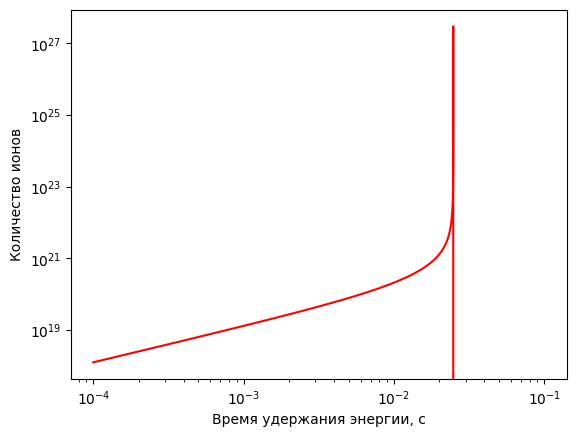
\includegraphics[width=0.5\textwidth]{"Graphs/Nbydt.png"}
	\caption{Зависимость допустимого объема от времени удержания плазмы}
\end{figure}\\
Откуда получаем, что время удержания плазмы $\tau \in [0.01; 0.05]$ с. Это дает связь между скоростью протекания ионов по камере и её длиной. 
\subsection{Реакционные блок и блок удержания}
Этот блок будет камерой, в которой будет достигаться:
\begin{enumerate}
	\item Огромное магнитное поле для защиты корпуса камеры. 
	\item большая концентрация ионов для более активного протекания реакции. 
	\item 
\end{enumerate} 
\end{document}